\section{Development view}
De development view is gefocust op het inbeeldt brengen van de organisatie van software modules en de software development omgeving \parencite{4+1ViewModelPaper}.
Om dit in beeld te brengen is er gebruikgemaakt van een component diagram (zie figuur \ref{fig:ComponentDiagram}).

% \todo[inline]{Ik ben het meest onzeker over dit diagram. Want ik heb een gevoel dat ik het veel te erg gegeneraliseerd heb.}

\whitespace[2]
\begin{graphic}
    \captionsetup{type=figure}
    \caption{Deployment diagram van het afstudeer product}
    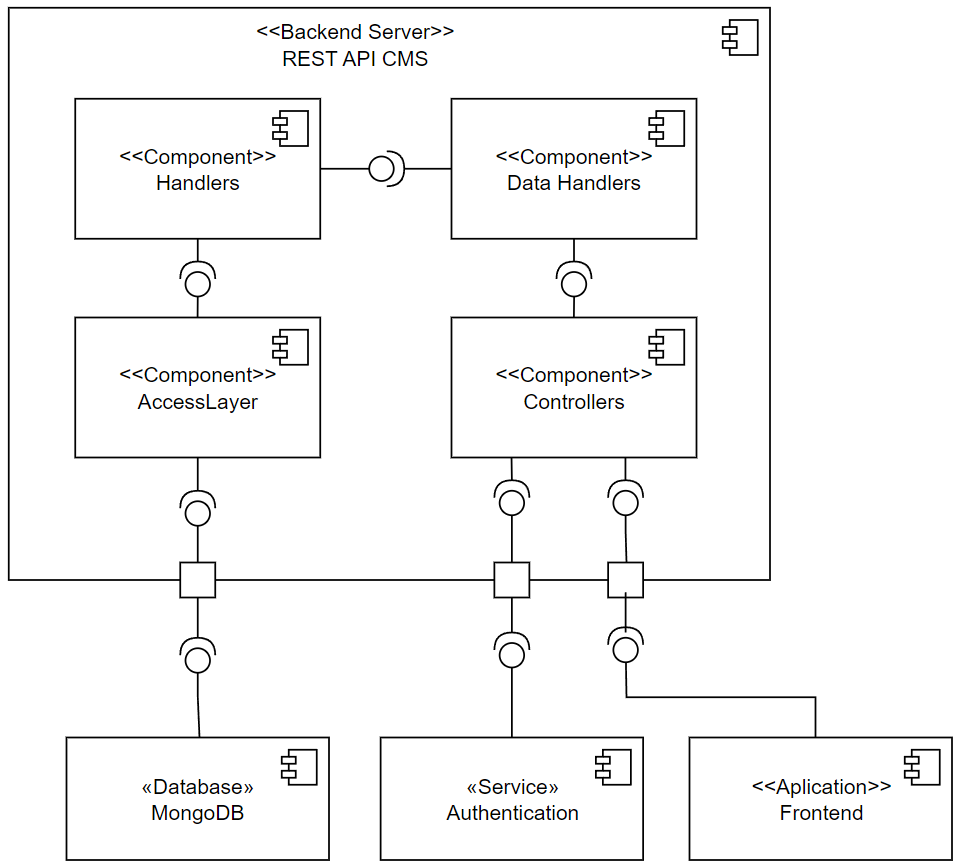
\includegraphics[scale=0.4]{ComponentDiagram.png}
    \label{fig:ComponentDiagram}
\end{graphic}


